
\documentclass[12pt]{article}

\usepackage{graphicx}
\graphicspath{ {./images/} }

\usepackage{epsfig}
\usepackage{amsmath,amsthm}
\usepackage{listings}


\newtheorem{lemma}{Lemma}
\newtheorem{theorem}{Theorem}


\usepackage{titlesec}
\titleformat{\section}
{\normalfont\Large\bfseries}{Question~\thesection:}{1em}{}

\newlength{\toppush}
\setlength{\toppush}{2\headheight}
\addtolength{\toppush}{\headsep}


\def\subjnum{Comp 160}
\def\subjname{Algorithms}


\def\doheading#1#2#3{\vfill\eject\vspace*{-\toppush}%
  \vbox{\hbox to\textwidth{{\bf} \subjnum: \subjname \hfil Erli Cai}%
    \hbox to\textwidth{{\bf} Tufts University, Fall 2020 \hfil#3\strut}%
    \hrule}}


\newcommand{\htitle}[1]{\vspace*{1.25ex plus 1ex minus 0ex}%
\begin{center}
{\large\bf #1}
\end{center}} 



\begin{document}
\doheading{2}{title}{Homework 00}
\setlength\parindent{0pt}


\section{}

(a) It is not good that we never resize the hash table because as the number of objects we hashed increases 1) For chaining method, the load factor, $\alpha$, increase, and time taken for search ($\theta(1+\alpha)$) increases accordingly. 2) For open addressing method, when the number of object we want to hash is more than the number of buckets, we will not able to find a bucket to put them.\\

(b)
Chaining method:\\
\begin{center}
 \begin{tabular}{||c c c c c c c c c c c||} 
 \hline
Bucket & 0 & 1 & 2 &3&4&5&6&7&8&9 \\ [0.5ex] 
 \hline\hline
 Numbers & 10 & &32 &23 &4 &35&26, 56&97&& \\ 
 \hline
\end{tabular}
\end{center}
Successful search: worst value case query time would be 3 steps(1 step for calculating hash value, 2 steps to search), for element 56.\\
Unsuccessful search: worst value case query time would be 4 steps(1 step for calculating hash value, 3 steps to search), for element 76.\\
For a unsuccessful search, we would have:
\begin{center}
 \begin{tabular}{||c c c c c c c c c c c||} 
 \hline
numbers ending in & 0 & 1 & 2 &3&4&5&6&7&8&9 \\ [0.5ex] 
 \hline\hline
 Numbers of Comparison & 1 & 0&1 &1 &1 &1&2&1&0&0 \\ 
 \hline
 \end{tabular}
\end{center}
Under the assumption of SUH, each key appears with same probability, So the average number of key comparisons needed $= \frac{1}{10}(1 + 0+1 +1 +1 +1+2+1+0+0 ) = 0.8$

Open addressing method:\\
\begin{center}
 \begin{tabular}{||c c c c c c c c c c c||} 
 \hline
Bucket & 0 & 1 & 2 &3&4&5&6&7&8&9 \\ [0.5ex] 
 \hline\hline
 Numbers & 10 & &32 &23 &4 &35&26&97&56& \\ 
 \hline
\end{tabular}
\end{center}
Successful search: worst value case query time would be 4 steps(1 step for calculating hash value, 3 steps to search), for element 56.\\
Unsuccessful search: worst value case query time would be 9 steps(1 step for calculating hash value, 8 steps to search), for element 42.\\
For a unsuccessful search, we would have:
\begin{center}
 \begin{tabular}{||c c c c c c c c c c c||} 
 \hline
numbers ending in & 0 & 1 & 2 &3&4&5&6&7&8&9 \\ [0.5ex] 
 \hline\hline
 Numbers of Comparison & 1 & 0&7 &6 &5 &4&3&2&1&0 \\ 
 \hline
 \end{tabular}
\end{center}
Under the assumption of SUH, each key appears with same probability, So the average number of key comparisons needed $= \frac{1}{10}( 1 + 0+7 +6 +5 +4+3+2+1+0) = 2.9$\\

(c) Because Chaining method require much more memory.

(d) Chaining: each buck is a pointer to an array(could be an empty array), so it takes m units of memory. And n element is stored in these arrays, so it occupied n units of memory. It sums up to n+m units of memory.\\
Open addressing: n elements are stored in a chaining table of size m. Assuming empty buckets still takes 1 unit memory, then it need a total of m units of memory.\\

(e) Open addressing table should have size m+n

(f)
Open addressing method:\begin{center}
 \begin{tabular}{||c c c c c c c c c c c c c c c c c c c||} 
 \hline
Bucket & 0 & 1 & 2 &3&4&5&6&7&8&9 &10&11&12&13&14&15&16&17\\ [0.5ex] 
 \hline\hline
 Numbers &  & &56 & &4 &23&&97&26& &10&&&&32&&& 35 \\ 

\end{tabular}
\end{center}
Successful search: worst value case query time would be 2 steps(1 step for calculating hash value, 1 steps to search), for element 56(actually any element takes same time).\\
Unsuccessful search: worst value case query time would be 3 steps(1 step for calculating hash value, 2 steps to search), for element 7.\\
For a unsuccessful search, we would have:
\begin{center}
 \begin{tabular}{||c c c c c c c c c c c||} 
 \hline
numbers in modulo 18 & 0 & 1 & 2 &3&4&5&6&7&8&9 \\ [0.5ex] 
 \hline\hline
 Numbers of Comparison & 0 & 0&1 &0 &2 &1&0&2&1&0 \\ 
 \hline
 numbers in modulo 18 & 10 & 11 & 12 &13&14&15&16&17&& \\ [0.5ex] 
 \hline\hline
 Numbers of Comparison & 1 & 0&0 &0 &1 &0&0&1&& \\ 
 \hline
 \end{tabular}
\end{center}
Under the assumption of SUH, each key appears with same probability, So the average number of key comparisons needed $= \frac{1}{18}(0 + 0+ 1+0 +2 +1+0+2+1+0+ 1 + 0+0 +0 +1 +0+0+1) = 0.5$\\
Conclusion, open addressing method perform better than chaining method if same amount of memory is used for both method



\pagebreak
\section{}

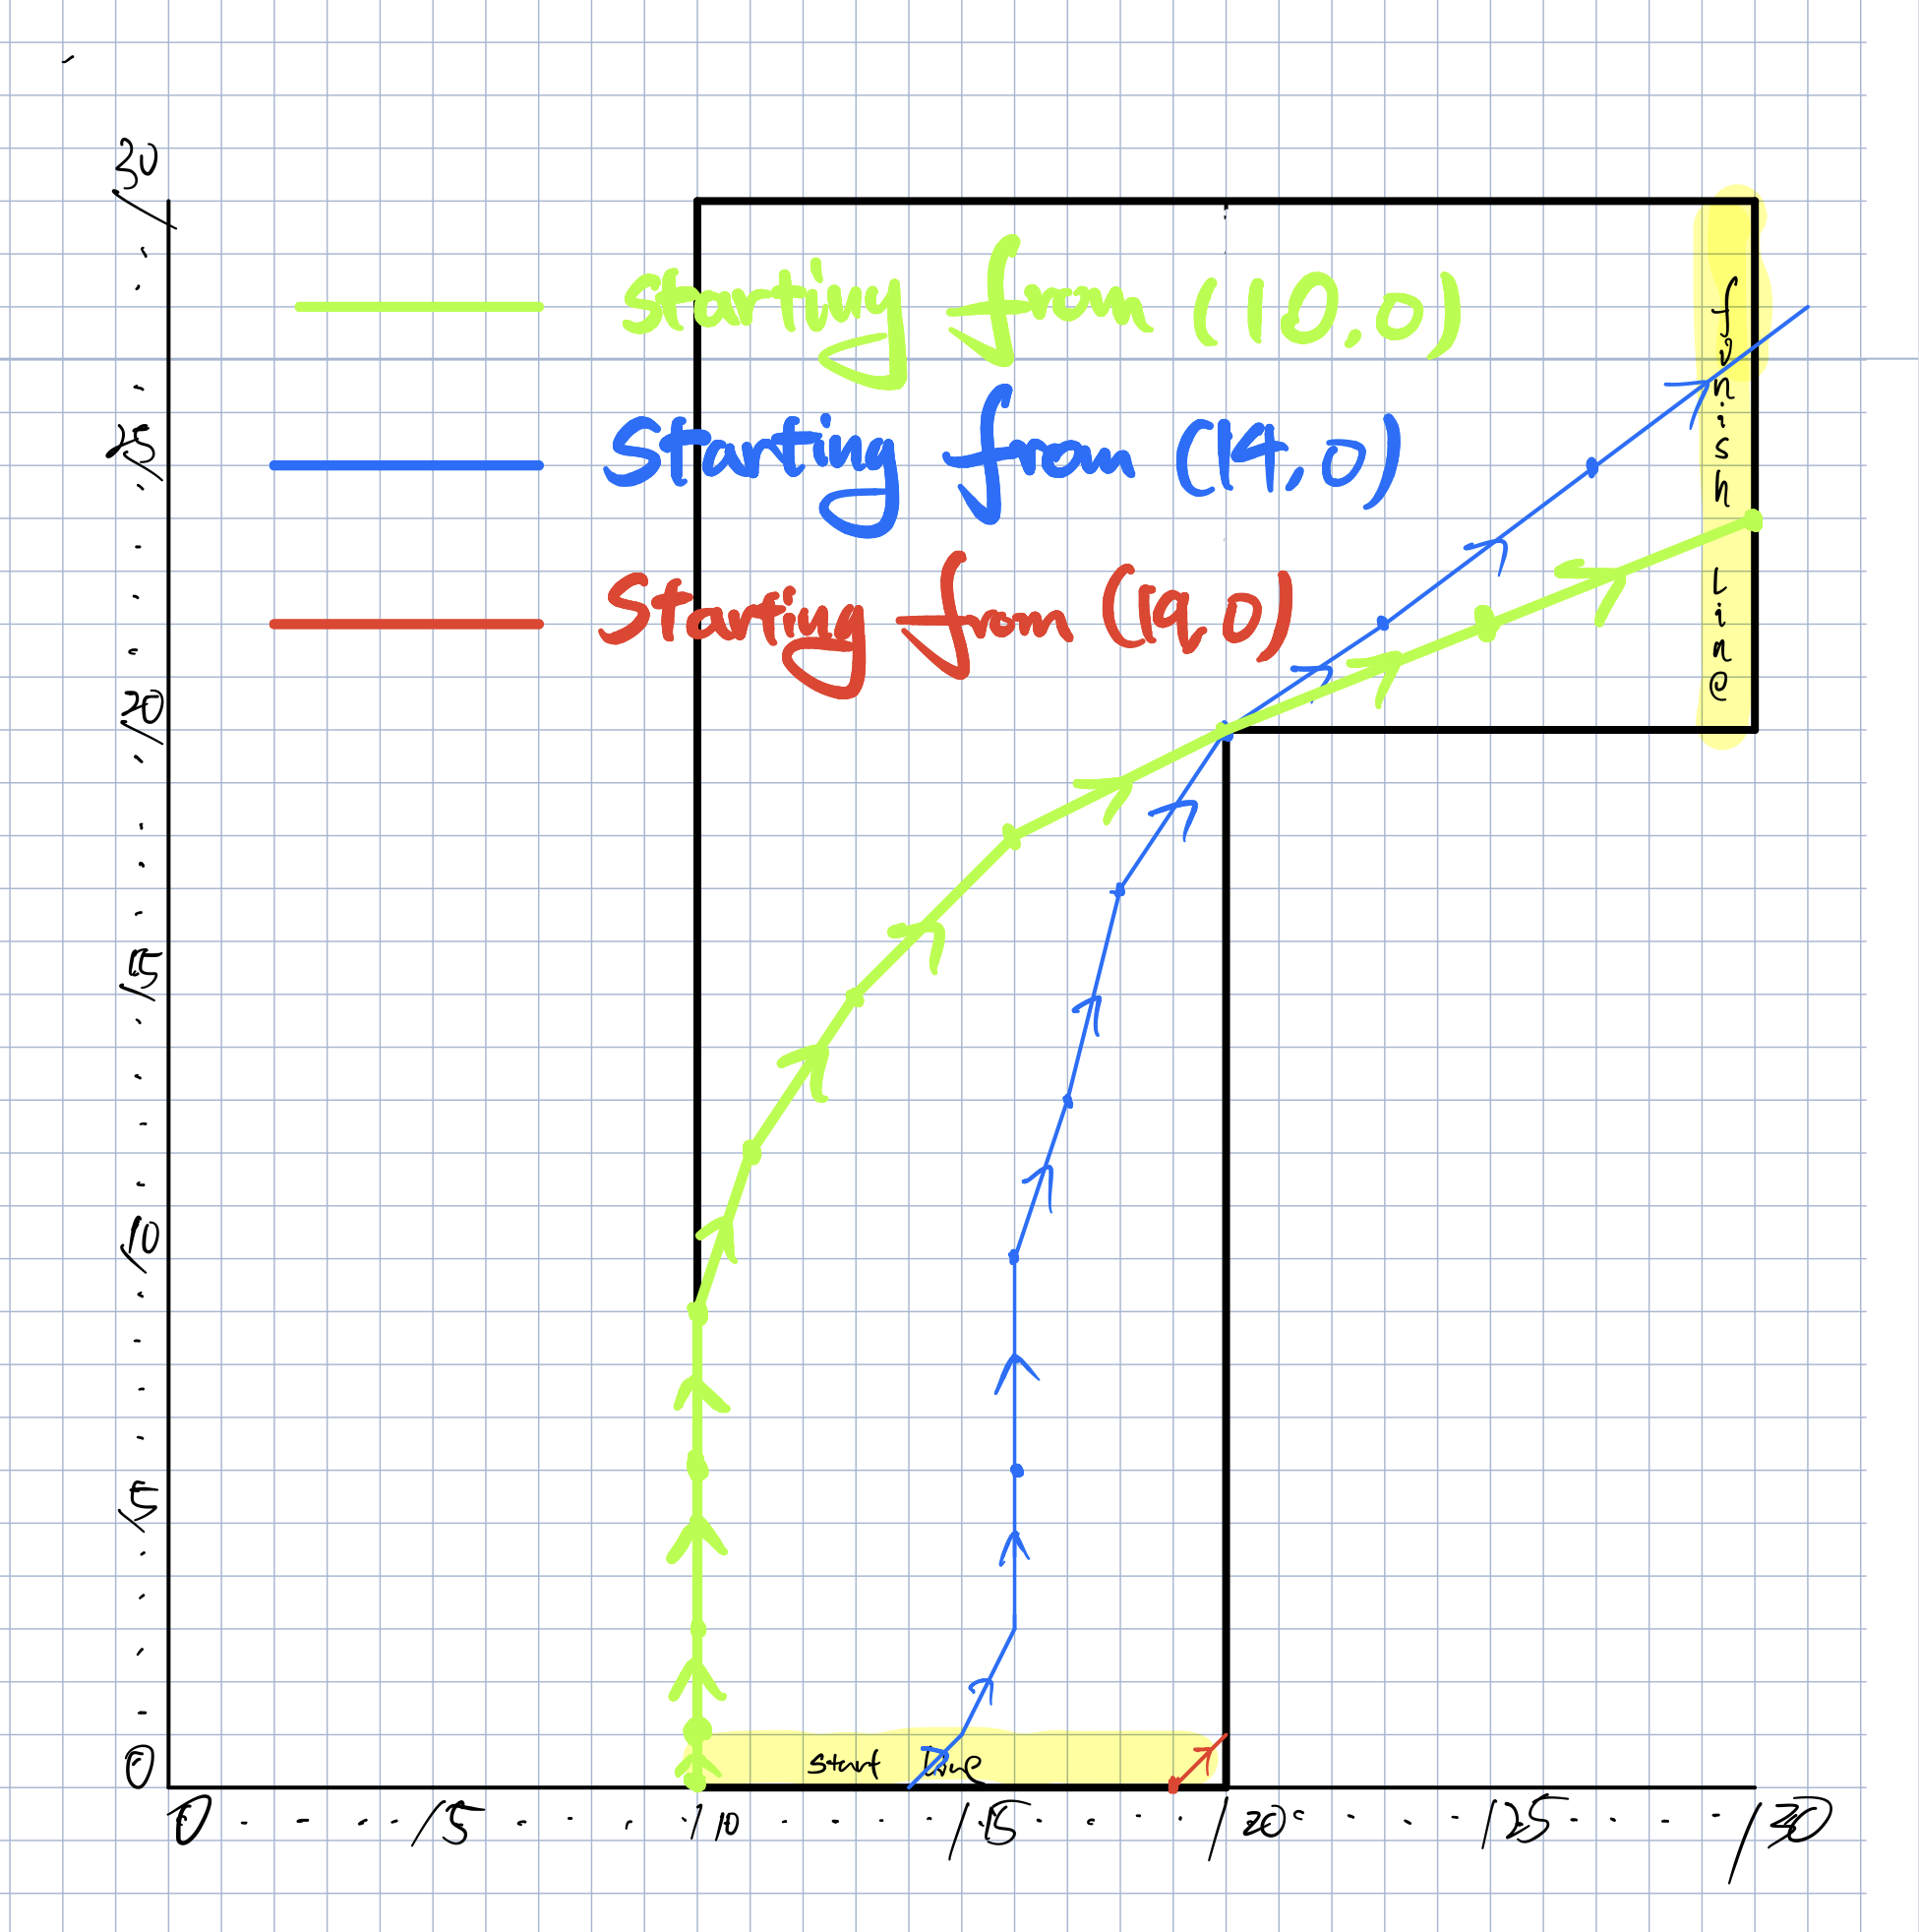
\includegraphics[scale = 0.15, angle = 270]{3.jpg}


\pagebreak
\section{}
I would use 2 AVL trees and a hashing table to handle these operations. One AVL tree (Let's call it Tree1 in later reference) storing addresses and id of datas occupying B units of memory sorting in terms of addresses. And one tree (Tree2) storing addresses and id of data occupying 2B units of memory sorting in terms of addresses. The hash table will store (id, address) pairs using id as key and use chaining method to resolve collision. Also, let the hash table be large enough so that loading factor($\alpha$) $<=$ 0.75.

\textbf{Initialise}:  Initialisation is just initialisation of 2 AVL trees and 1 hash table, so $\theta(1)$ time needed

\textbf{InsertBlock (id, address, length)}: In each insertion, we would need to insert one (id, addresses) pair in hash table $(\Theta(1+\alpha) $time). And depending on length, we will insert a value into either Tree1 or Tree2 ($\Theta(h)$time where h is the height). Assuming we have n blocks of data we want to store in our DS, the each insertion would cost $\Theta(\log n)$ time

\textbf{DeleteBlock (id)}: we search for the corresponding addresses using our hash table. If search is unsuccessful, send error message. If search is successful, then searching for that address in the both AVL tree(since we don't know which one it will be in). Then delete the address from AVL tree and delete (id, address) pair in hash table.\\
Searching in hash table cost $\Theta(1+\alpha)$ time. searching in each AVL tree takes $\Theta(h)$time. Assuming we have inserted n blocks of data in our DS, the each deletion would cost $\Theta(\log n)$ time

\textbf{FindBlock (queryAddress)}:  Search for the largest address in each AVL tree that is less than queryAddress. Assume we get a1 from Tree1 and a2 from Tree2. if $ a1 \le queryAddress \le a1+B$, then return corresponding id of a1. if $ a2 \le queryAddress \le a2+2B$, then return corresponding id of a2. If neither of the above is true, then no block is occupying that position. Assuming n elements in stored in AVL trees,two search in AVL tree is required, so $\Theta(\log n)$ runtime.

Correctness: Since we are using AVL trees and hash table in our DS, the correctness is justified by the correctness of AVL tree and hash table.


\end{document}


